\section{Durchführung}
\label{sec:Durchfuehrung}

Für alle Messungen wurde eine Drillachse verwendet.
Sie besteht aus einer senkrecht gelagerten Achse, die über eine Spiralfeder mit dem Rahmen verbunden ist.
Um die Achse herum ist eine Winkelskala in Grad angebracht, an der die Auslenkung abgelesen werden kann.
Die untersuchten Körper wurden direkt auf die Achse gesteckt bzw. mit einer Rändelschraube in ihr festgeklemmt (siehe \autoref{fig:haltungen}).
Um die Spiralfeder nicht inelastisch zu verformen, wurde die Achse nie weiter als $360^\circ$ ausgelenkt.
Zeiten wurden mit der Stoppuhr eines Smartphones gemessen, Längen mit einem Rollmaßband und Massen mit einer Digitalwaage.

\subsection{Bestimmung der Winkelrichtgröße}
\label{sec:durchf_D}

% Winkelbereich (40° bis 140°) noch mit den Messdaten des Partners abgleichen!
Zur statischen Bestimmung von $D$ wurde eine leichte Metallstange auf die Drillachse gesteckt
und im Abstand $r = \qty{20}{\centi\metre}$ von der Drehachse eine Federwaage an ihr eingehängt.
Mit der Federwaage wurde die Achse um den Winkel $\varphi$ ausgelenkt.
Die Federwaage wurde dabei senkrecht zum Radius gehalten, damit die Kraft senkrecht zum Hebelarm wirkt und \autoref{eq:winkelrichtgroesse} gilt.
Für elf verschiedene Winkel von $10^\circ$ bis $100^\circ$ in Schritten von $10^\circ$ wurde die Kraft $F$ an der Federwaage abgelesen.
Dabei wurde immer in dieselbe Richtung ausgelenkt, und der Abstand $r$ blieb bei allen Messungen gleich.

\subsection{Bestimmung des Eigenträgheitsmoments der Drillachse}
\label{sec:durchf_ID}

Zur Bestimmung von $I_\text{D}$ wurde ein Metallstab waagerecht auf die Drillachse gesteckt, auf dem zwei gleiche zylindrische Gewichte
symmetrisch zur Drehachse befestigt waren.
Der Stab und die beiden Gewichte wurden vorher gewogen.
Gemessen wurde der Abstand von der Drehachse bis zum inneren Rand der Gewichte.
Da die Gewichte $\qty{2}{\centi\metre}$ breit sind, wurde dazu jeweils $\qty{1}{\centi\metre}$ addiert,
sodass $a$ den Abstand der Schwerpunkte der Gewichte zur Drehachse angibt.

Die Achse wurde um $180^\circ$ ausgelenkt und losgelassen.
Anschließend wurde die Dauer der ersten beiden Perioden einzeln gestoppt.
Diese Messung wurde für zehn verschiedene Abstände zwischen $a = \qty{3}{\centi\metre}$ und $a = \qty{29}{\centi\metre}$ durchgeführt.
Bei $a = \qty{15}{\centi\metre}$ wurde zusätzlich eine Messung mit einer Auslenkung von $90^\circ$ durchgeführt,
um zu prüfen, ob die Periodendauer von der Auslenkung abhängt.

\subsection{Trägheitsmomente von Kugel und Zylinder}
\label{sec:durchf_koerper}

Untersucht wurden eine Holzkugel und ein Metallzylinder.
Beide wurden gewogen, und der Radius der Kugel sowie der Durchmesser des Zylinders wurden gemessen.
Die Körper wurden nacheinander direkt auf die Drillachse gesteckt, der Zylinder mit seiner Symmetrieachse parallel zur Drehachse.
Wie zuvor wurde jeweils um $180^\circ$ ausgelenkt und die Dauer der ersten beiden Perioden gestoppt.
Die Messung wurde für jeden Körper fünfmal durchgeführt.

\subsection{Trägheitsmoment der Holzpuppe}
\label{sec:durchf_puppe}

Zunächst wurde die Puppe gewogen.
Anschließend wurden die Durchmesser von Armen, Beinen, Rumpf und Kopf jeweils fünfmal gemessen,
sowie die Längen von Armen, Beinen und Rumpf.

Die Puppe ist auf einem dünnen Metallstab befestigt, der in die Drillachse eingespannt wurde.
Es wurden zwei Haltungen untersucht, die in \autoref{fig:haltungen} dargestellt sind.
In Haltung~1 waren Arme und Beine schräg vom Körper weggestreckt, die Arme zur Seite und die Beine nach vorne und hinten.
Hier wurde zusätzlich der waagerechte Abstand von Händen und Füßen zur Drehachse gemessen, um die Neigung der Gliedmaßen bestimmen zu können.
In Haltung~2 waren die Arme waagerecht ausgestreckt (T-Pose) und die Beine zeigten gerade nach unten.

Für jede Haltung wurde die Puppe um $180^\circ$ ausgelenkt und die Dauer der ersten beiden Perioden gestoppt.
Die Messung wurde für jede Haltung fünfmal durchgeführt.

\begin{figure}
    \centering
    \begin{subfigure}{0.45\textwidth}
        \centering
        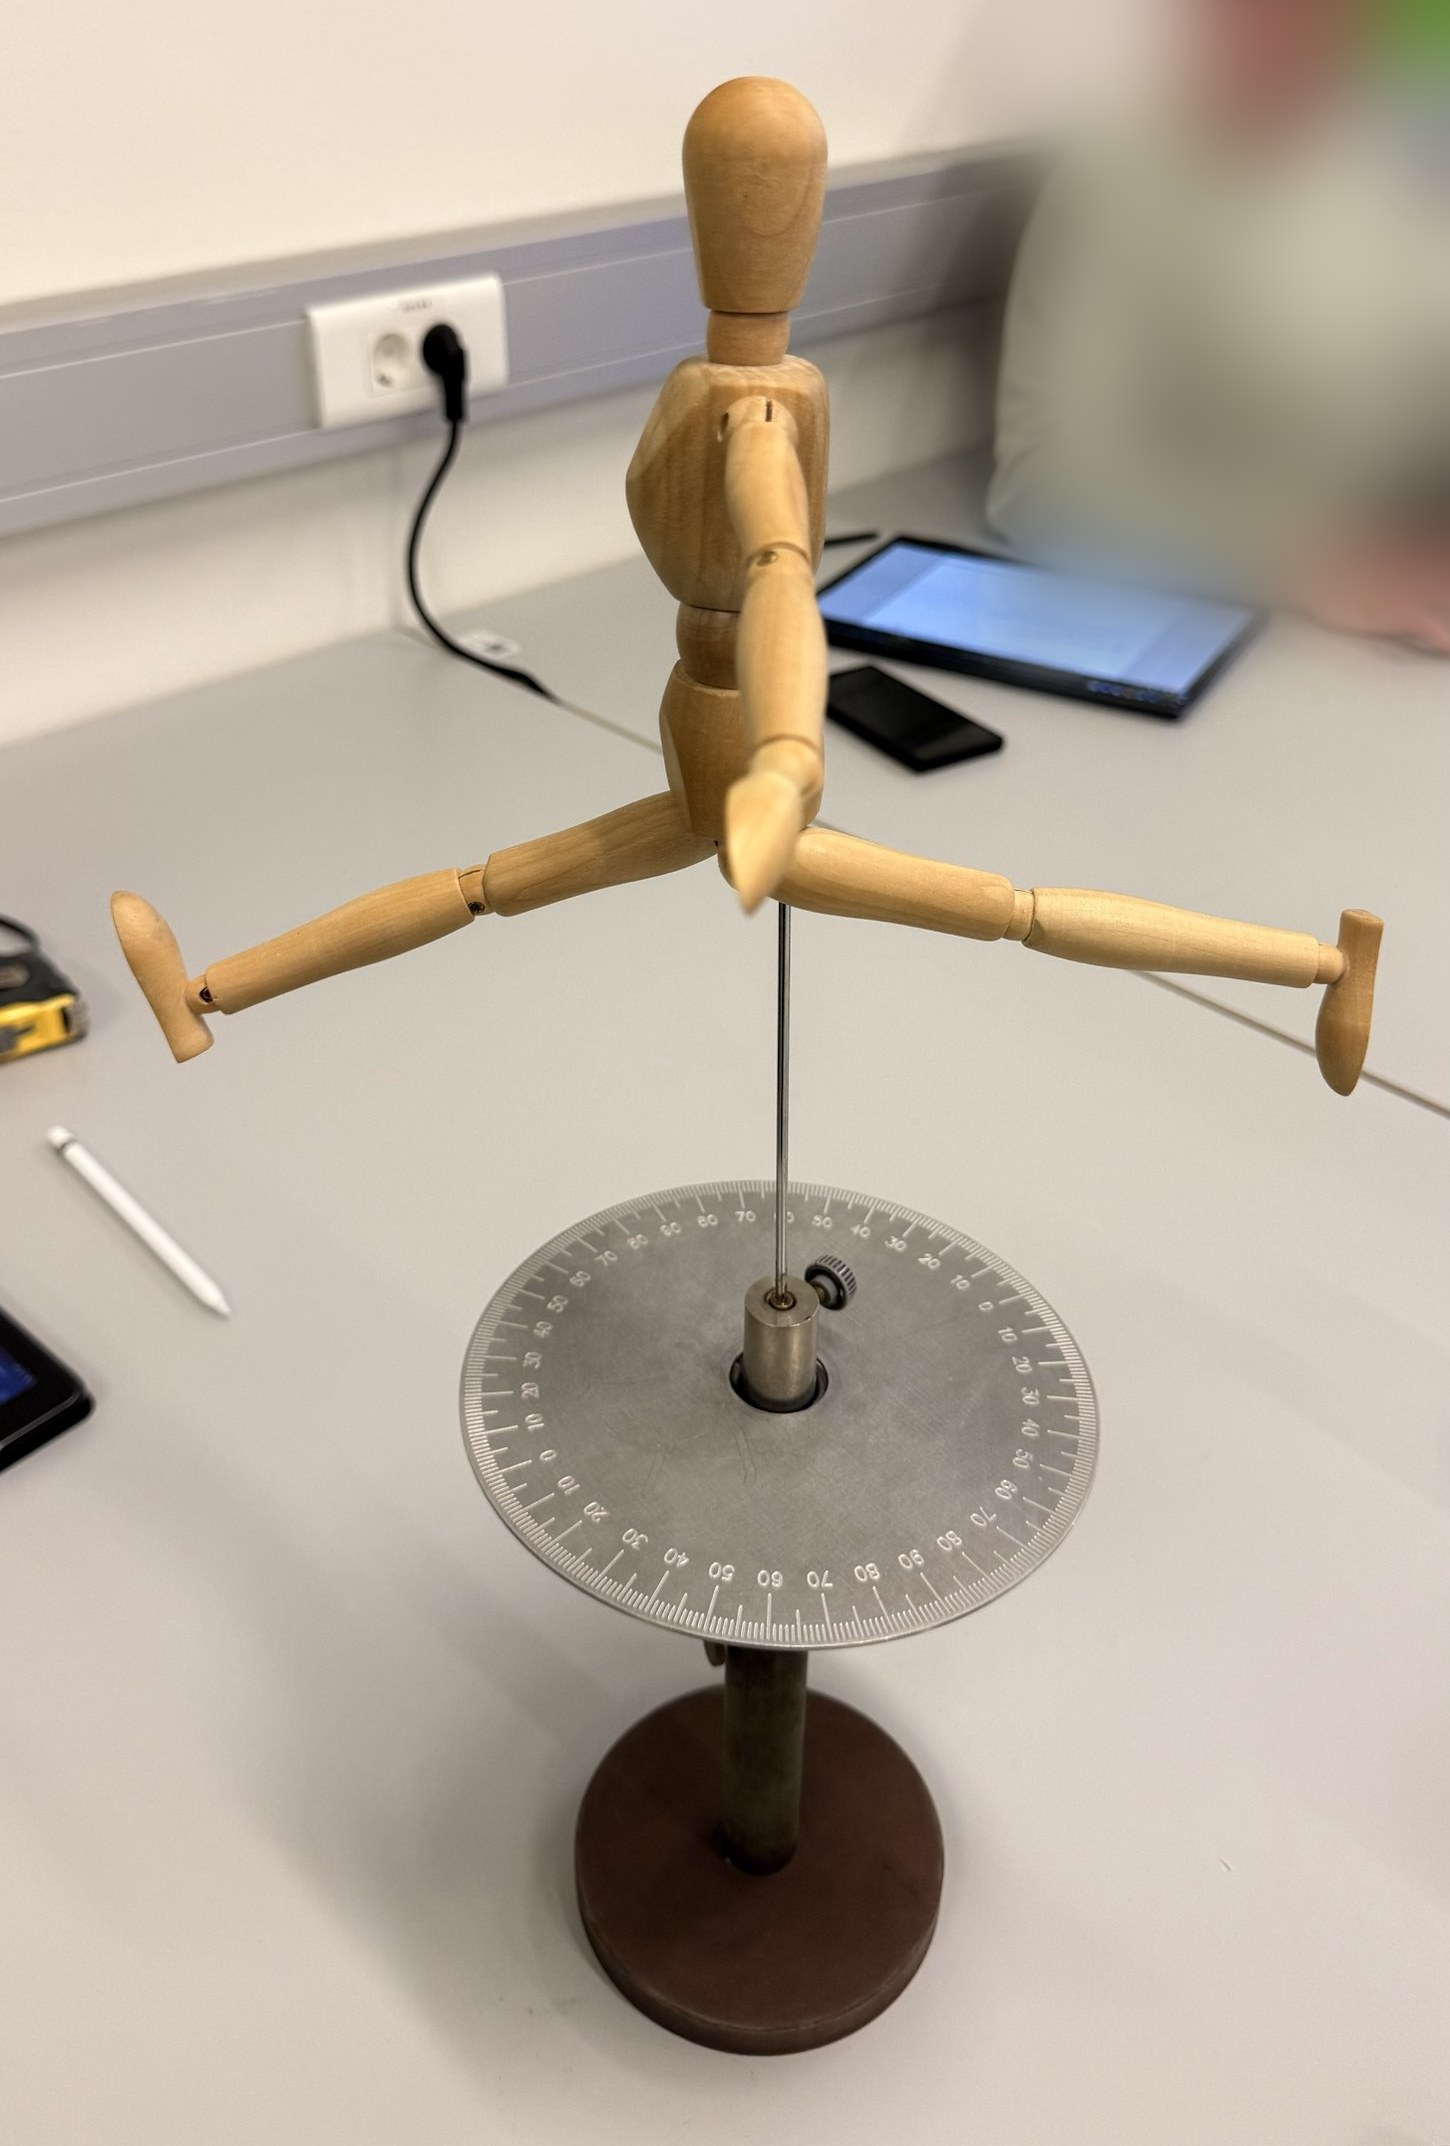
\includegraphics[width=\textwidth]{images/haltung1_seite.jpg}
        \caption{Haltung 1.}
        \label{fig:haltung1}
    \end{subfigure}
    \hfill
    \begin{subfigure}{0.45\textwidth}
        \centering
        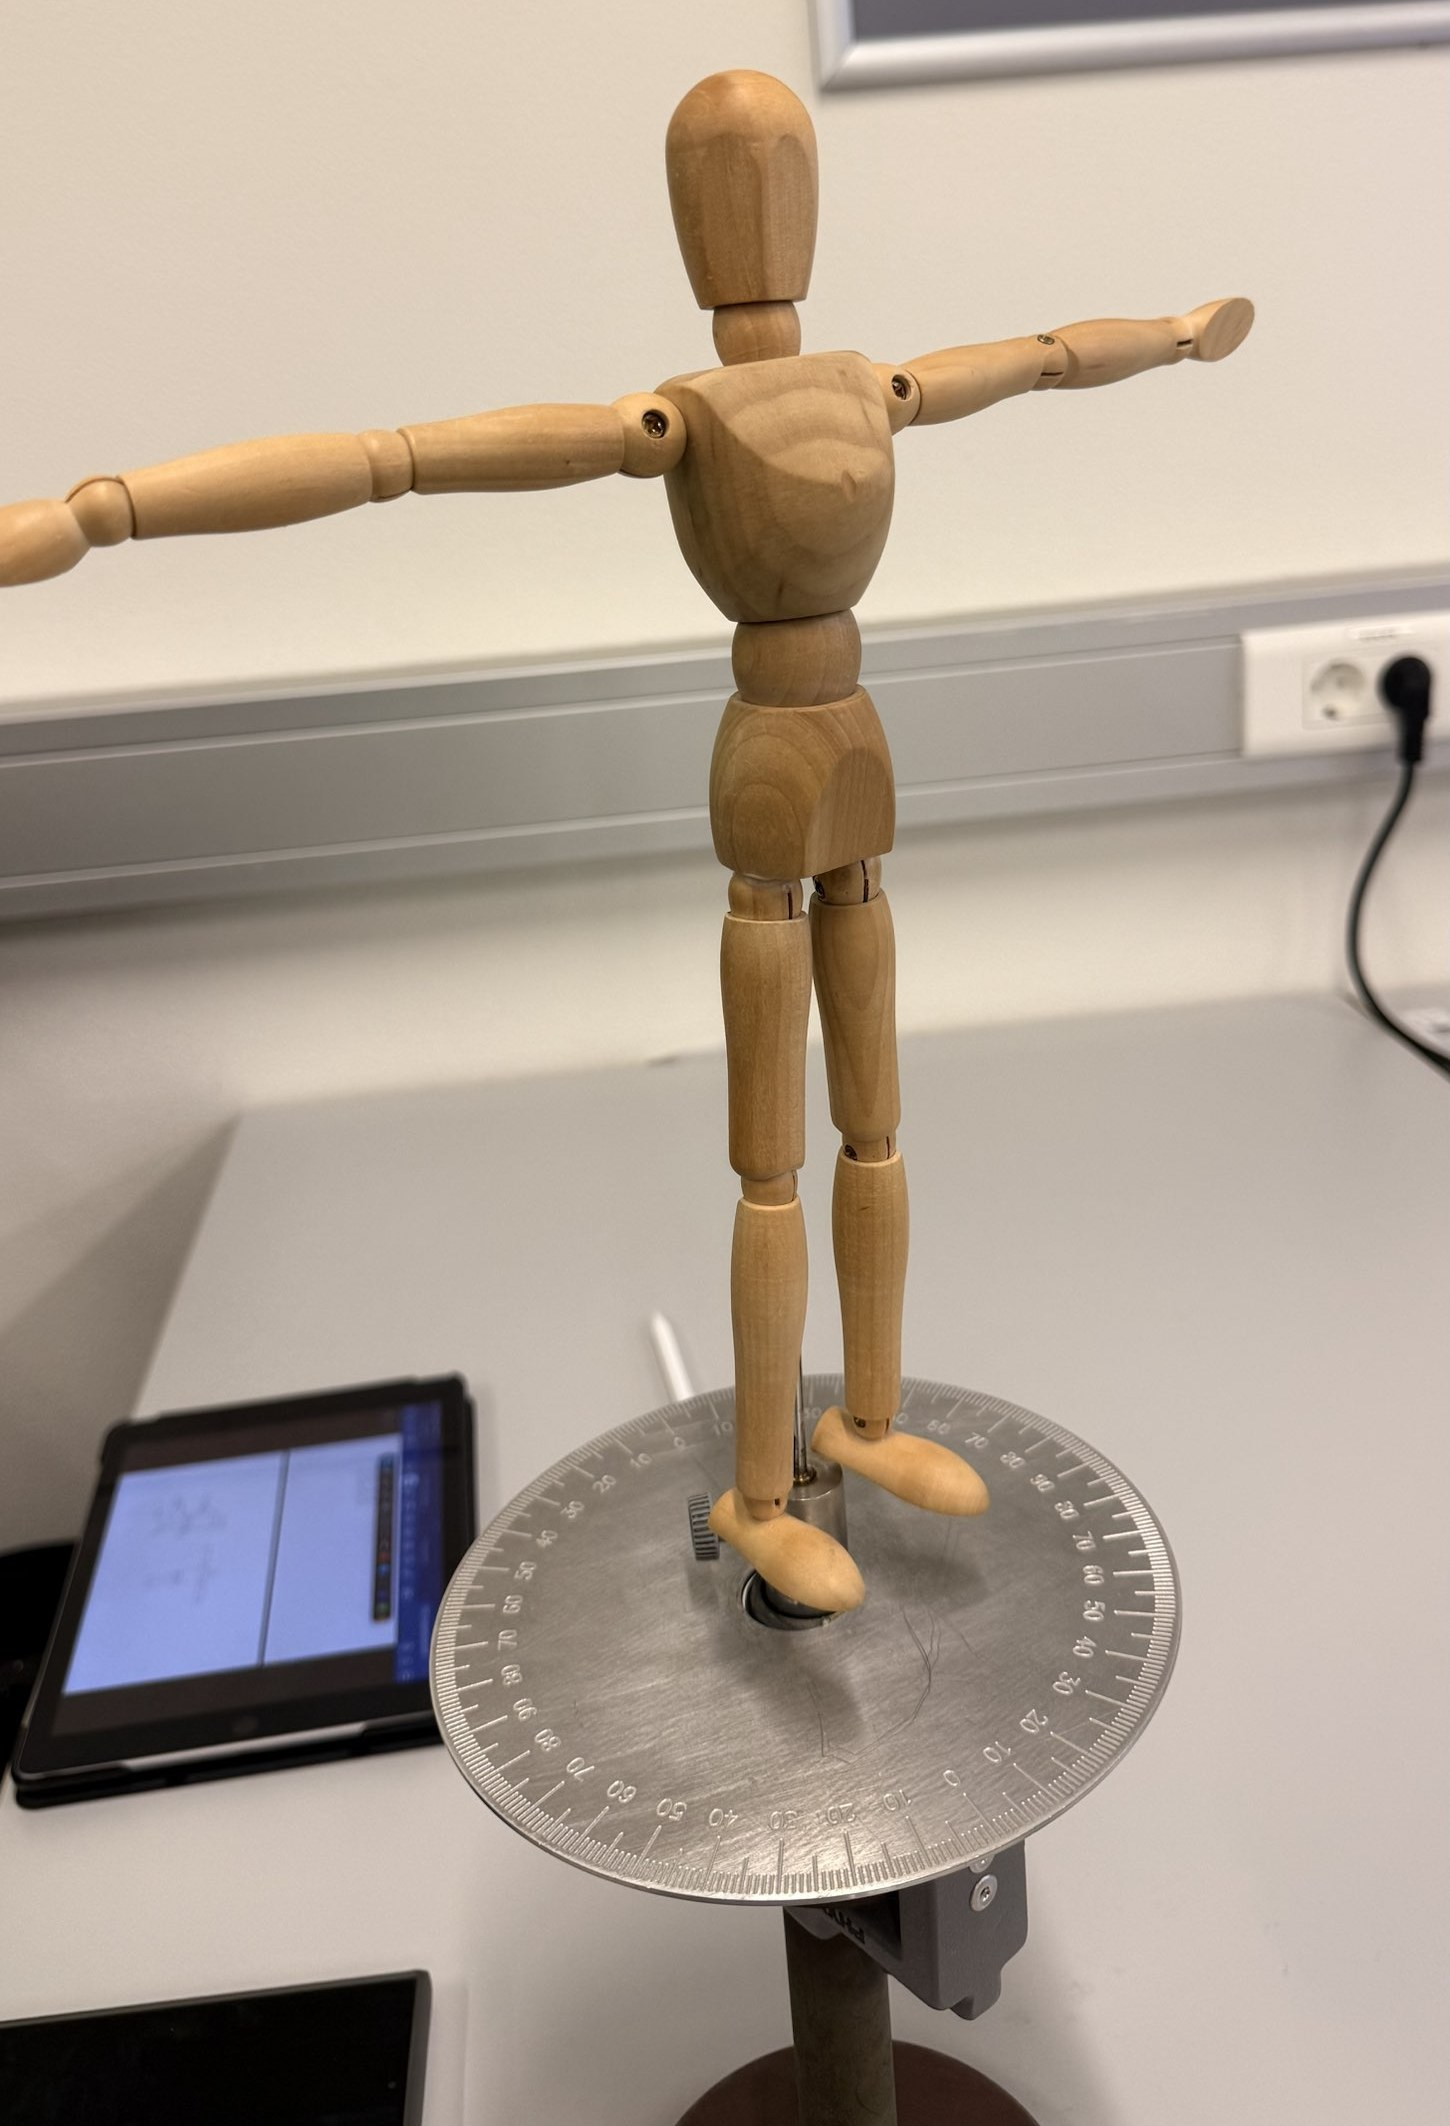
\includegraphics[width=\textwidth]{images/haltung2_vorne.jpg}
        \caption{Haltung 2 (T-Pose).}
        \label{fig:haltung2}
    \end{subfigure}
    \caption{Die Holzpuppe auf der Drillachse in den beiden untersuchten Haltungen.}
    \label{fig:haltungen}
\end{figure}